\newpage
\section{O que é \textit{blockchain}?}
\label{sec:blockchain_what}

Na sua aplicação mais básica é um conceito bastante simples de explicar:

``\textit{Blockchain é um tipo de Base de Dados Distribuída que guarda um registo de transações permanente e à prova de violação. Uma base de dados em blockchain consiste em dois tipos de registos: transações individuais e blocos.}

\textit{Um bloco é a parte concreta da blockchain onde são registadas algumas ou todas as transações mais recentes e uma vez concluídas são guardadas na blockchain como base de dados permanente. Sempre que um bloco é concluído um novo é gerado. Existe um número incontável de blocos na blockchain que são ligados uns aos outros - como uma cadeia - onde cada bloco contém uma referência para o bloco anterior.}'' \cite{blockchain_wiki}

Duma forma mais visual pode se usar o esquema referido na \cref{fig:blockchain-bitcoin-overview}, em que cada bloco contem o \textit{hash} do bloco anterior e a raiz da \textit{Merkle Tree}, que é uma árvore de \textit{hashs} para indexar o conteúdo.

\begin{figure}[!h]
  \centering
    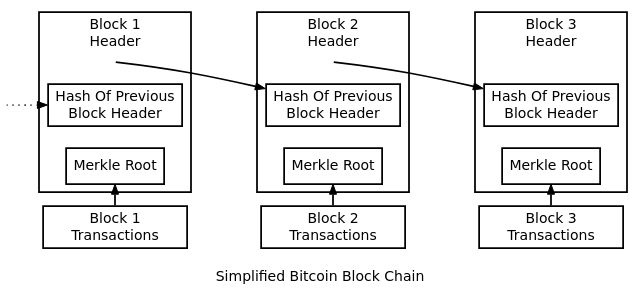
\includegraphics[width=0.9\textwidth]{bitcoin-blockchain-simplefied.png}
  \caption{Visão geral do \textit{blockchain} no \textit{Bitcoin} \cite{bitcoin_devguide_blockchain}}
 \label{fig:blockchain-bitcoin-overview}
\end{figure}

O conceito de \textit{blockchain} foi introduzido por David Chaum em 1982 \cite{blockchain_origem} e foi conceptualizado por uma pessoa ou grupo conhecido como "Satoshi Nakamoto" em 2008 que publicou o design e implementação do que hoje é conhecido como \textit{Bitcoin}. \cite{blockchain_nakamoto}